\clearpage
\section{对话案例展示}
\label{app:showcase}

图~\ref{fig:showcase_path_pmc}--\ref{fig:showcase_m3d}展示 CoEvoMed 对话案例，覆盖六个二维与三个三维基准。每个区块呈现视觉输入、用户问题与模型回答，GT 表示参考答案。

\begin{figure}[H]
\centering
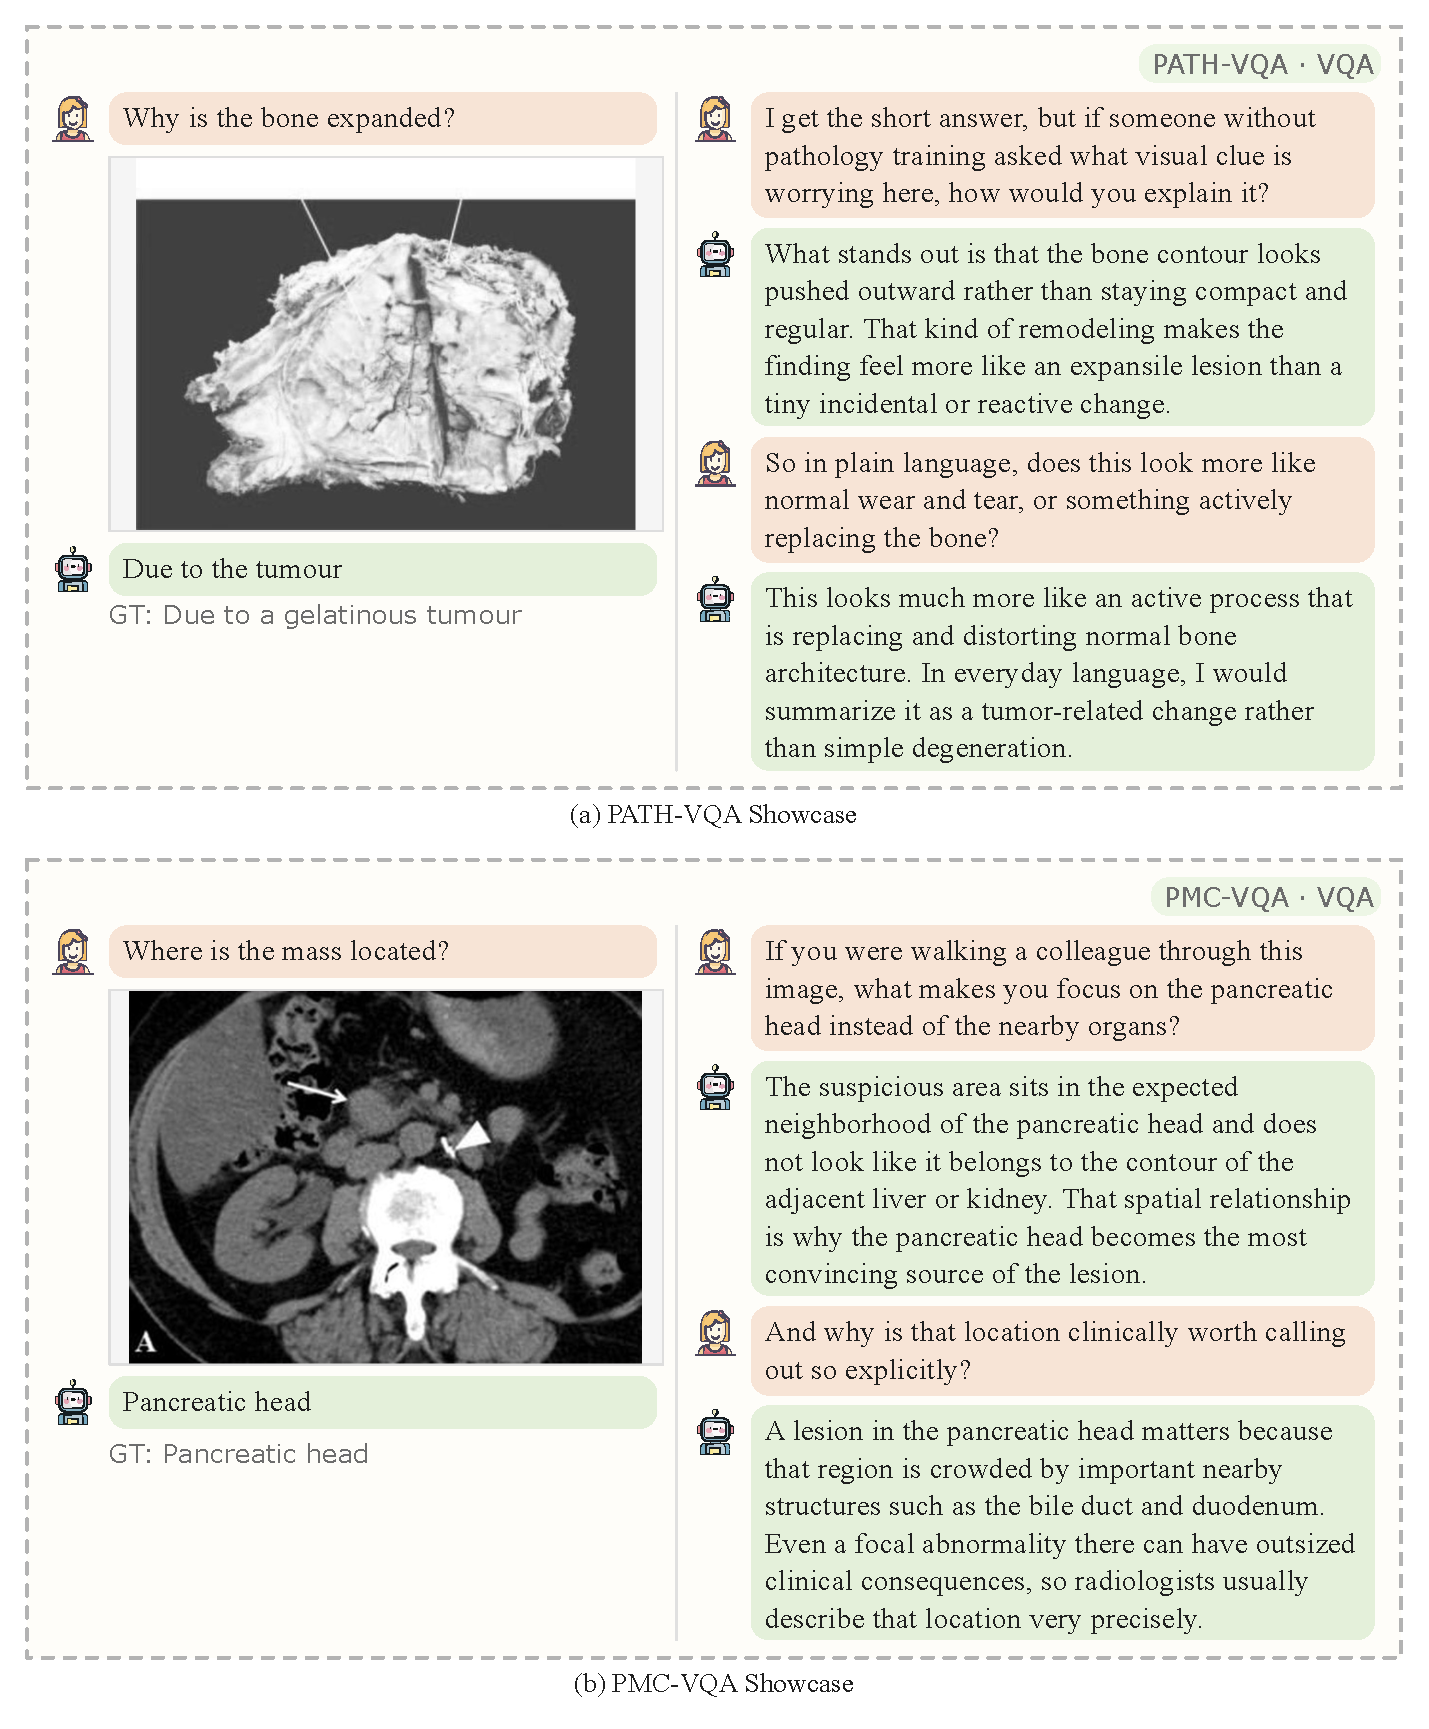
\includegraphics[width=\linewidth]{figures/showcase/medical_vqa_2d.pdf}
\caption{CoEvoMed 在 PathVQA（上）与 PMC-VQA（下）的多轮对话案例。}
\label{fig:showcase_path_pmc}
\end{figure}

\clearpage
\begin{figure}[H]
\centering
\includegraphics[page=2,width=\linewidth]{figures/showcase/medical_vqa_2d.pdf}
\caption{CoEvoMed 在 SLAKE（上）与 VQA-RAD（下）的多轮对话案例。}
\label{fig:showcase_slake_rad}
\end{figure}

\clearpage
\begin{figure}[H]
\centering
\includegraphics[page=3,width=\linewidth]{figures/showcase/medical_vqa_2d.pdf}
\caption{CoEvoMed 在 IU-Xray（上）与 MIMIC-CXR（下）的报告生成多轮对话案例。}
\label{fig:showcase_reports}
\end{figure}

\clearpage
\begin{figure}[H]
\centering
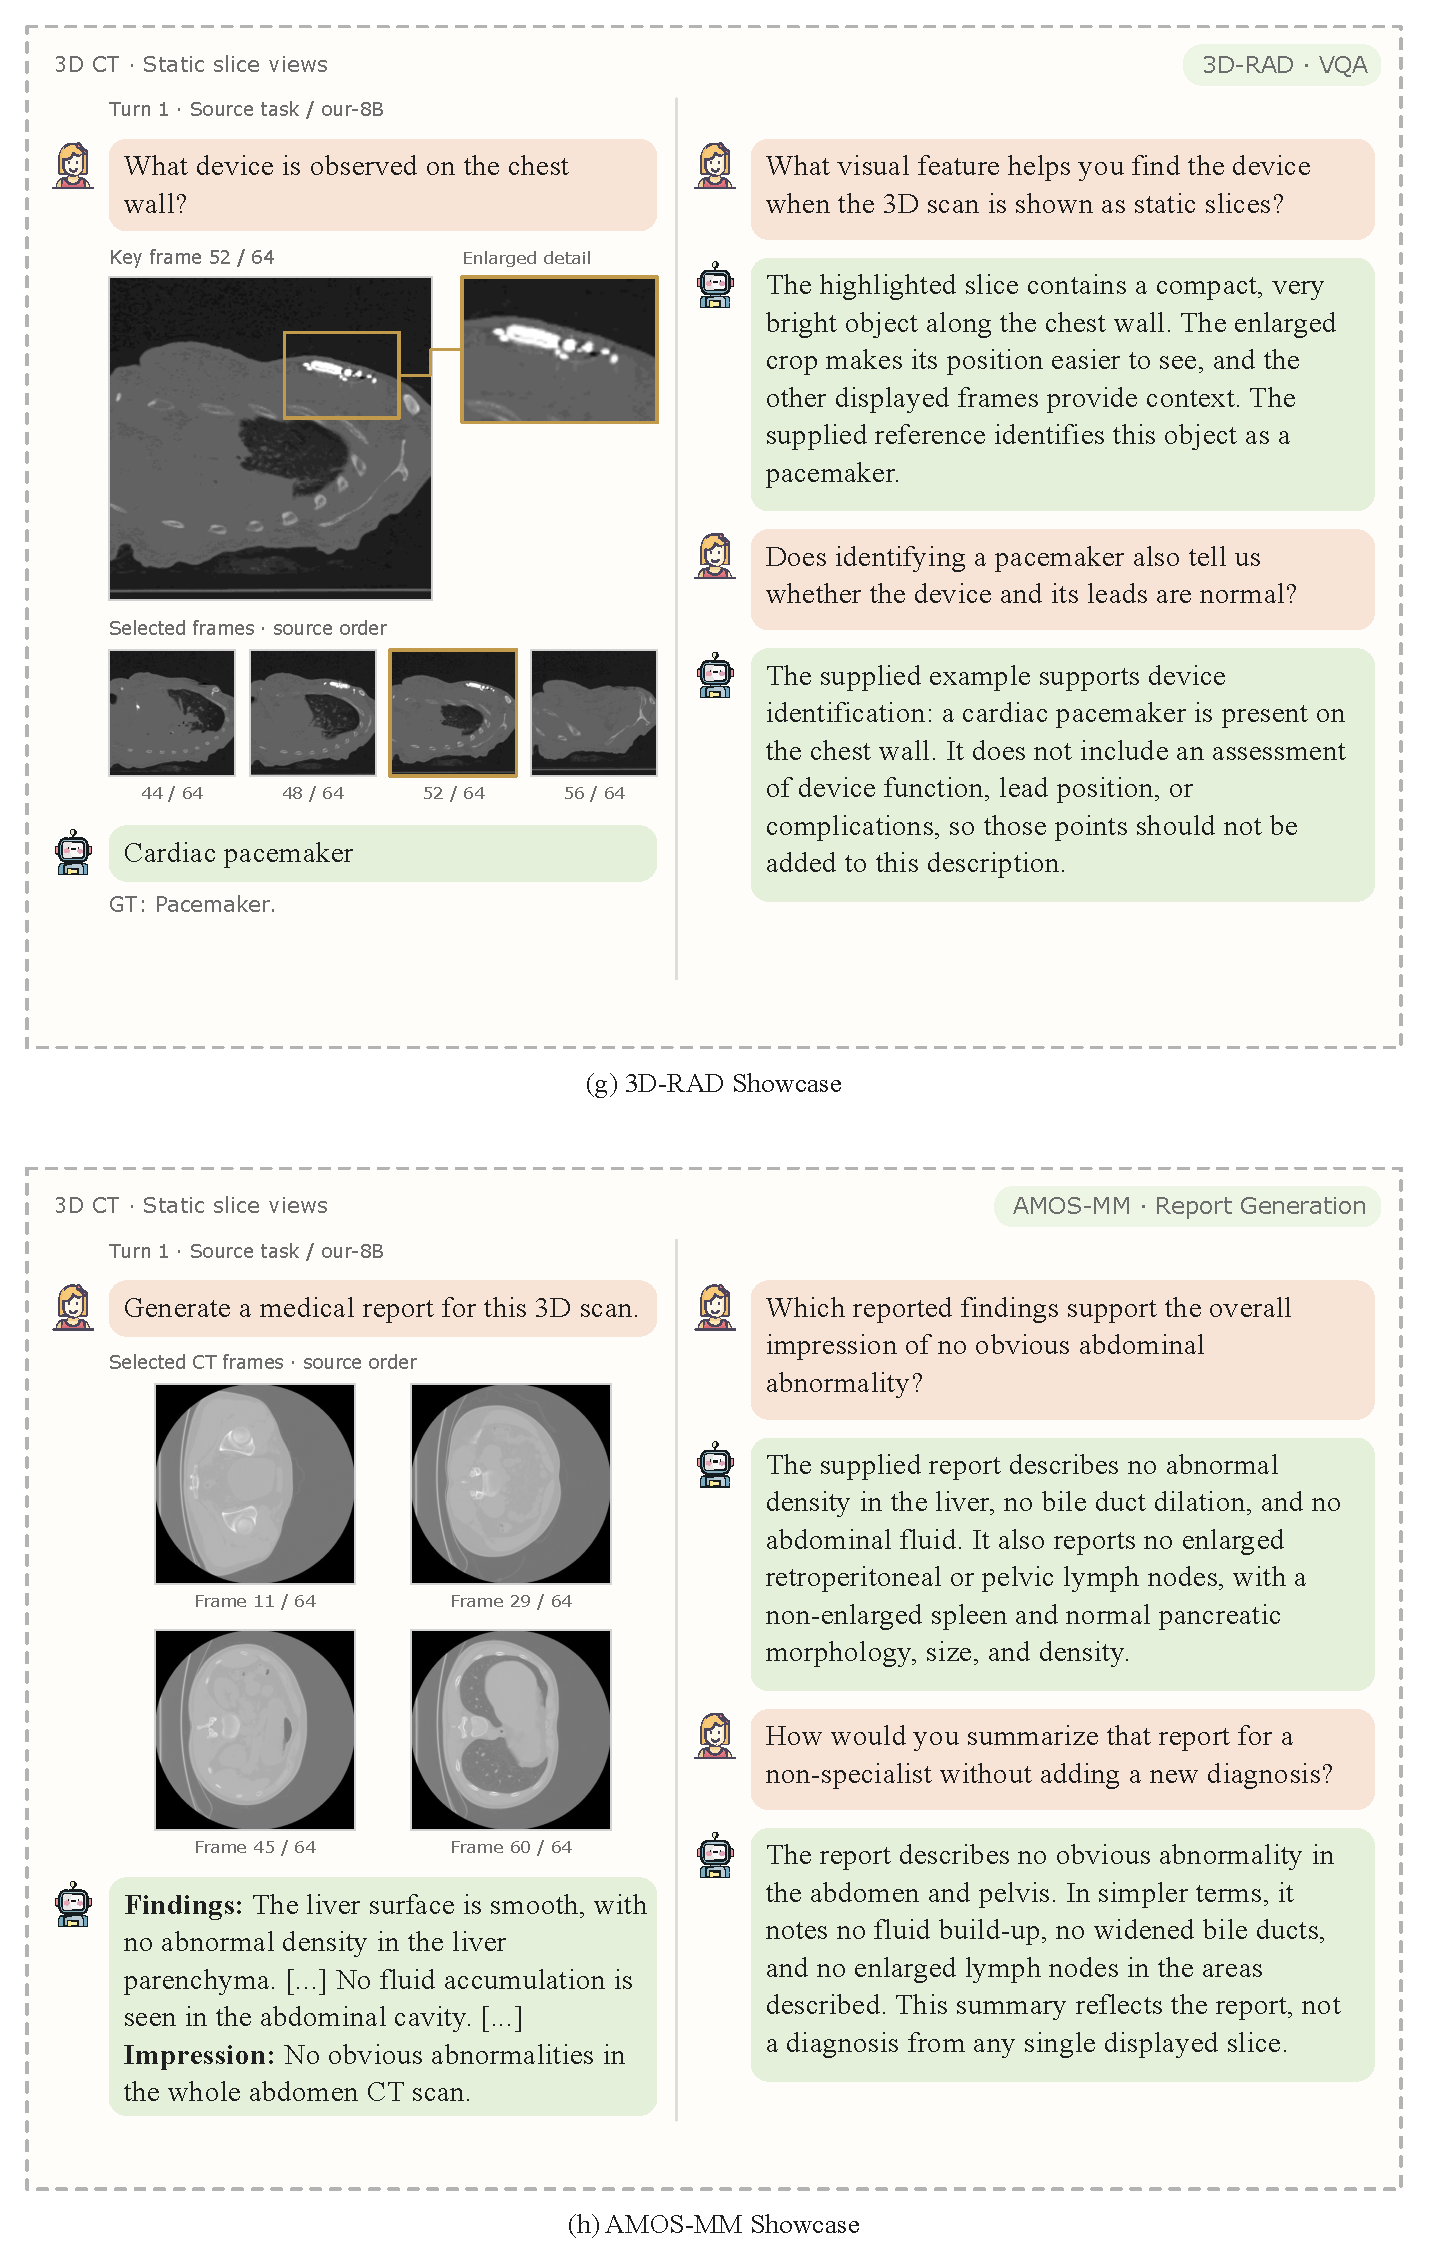
\includegraphics[width=\linewidth,height=0.86\textheight,keepaspectratio]{figures/showcase/medical_vqa_3d_pairs.pdf}
\caption{CoEvoMed 在 3D-RAD（上）与 AMOS-MM（下）的多轮对话案例及选定 CT 切片。AMOS-MM 报告以节选形式展示，省略号标记省略内容。}
\label{fig:showcase_rad_amos}
\end{figure}

\clearpage
\begin{figure}[H]
\centering
\includegraphics[page=2,width=\linewidth]{figures/showcase/medical_vqa_3d_pairs.pdf}
\caption{CoEvoMed 在 M3D-VQA 上的多轮对话案例、选定 CT 切片及局部放大图。}
\label{fig:showcase_m3d}
\end{figure}
